\section{Introduction} 
\label{sec:intro}

\textcolor{red}{In many real-world scenarios, decision-makers are required to make a series of choices over time, with the goal of optimizing a long-range objective and without knowing the outcomes in advance. Such sequential decision-making processes (also known as online learning) are prevalent in various fields such as finance~\citep{bell1988game, ban2018machine}, healthcare~\citep{bastani2021efficient, killian2023robust}, and online advertising~\citep{wagner2019digital, choi2020online}. For instance, a financial portfolio manager must decide which assets to invest in daily, balancing potential returns against risks. Similarly, a doctor might choose a treatment plan for a patient, adjusting it based on the response over time. In online advertising, companies continuously select which ads to display to users to maximize engagement and revenue.}

\textcolor{red}{There are two dominant models on the nature of the environment generating the data: stochastic or adversarial. In a stochastic environment, the data is assumed to be generated from an unknown, but fixed probability distribution. This assumption allows for the use of statistical methods to predict future outcomes based on historical data, making it possible to optimize decisions under uncertainty. For example, in finance, asset prices might be modeled using stochastic processes to forecast future market trends. Conversely, in an adversarial environment, the data is assumed to be generated by an adversary who aims to thwart the decision-maker’s efforts. This assumption is crucial in scenarios where the decision-maker faces strategic manipulation or worst-case scenarios. Such adversarial models ensure that decision-making strategies remain robust and perform well even when faced with the most challenging and unpredictable conditions, making them ideal for use in high-stakes applications where robust guarantees on performance are important.}

\textcolor{red}{Usually, the environment is a-priori assumed to follow one of these two models, and consequently decision-making strategies are designed for optimal performance in the assumed environment. Strategies designed for stochastic environments are typically simple to deploy and can achieve excellent performance for most outcome sequences, they are extremely vulnerable to strategic attacks, where an adversary can exploit their predictability and cause significant losses. On the other hand, worst-case optimal strategies offer stronger guarantees against adversarial manipulation, ensuring robust performance even in the most challenging scenarios. This duality in the strengths and weaknesses of the two aforementioned approaches highlights the need for algorithms that can seamlessly adapt to both benign and adversarial conditions. Such a need is also practically relevant; for instance, in~\cite{bastani2021mostly} it is shown that simple greedy algorithms work effectively for most typical data in a certain contextual bandit setting, both theoretically and empirically on healthcare datasets. However, in healthcare, robustness is crucial to ensure reliable performance across diverse and unpredictable patient responses. This underscores the necessity for “best of both worlds” methods that can leverage the simplicity and efficiency of stochastic strategies while retaining the robustness of worst-case optimal strategies---the problem we study in this paper. 
}

\subsection{Formal setup}

Our work aims to develop algorithms for online learning that are \emph{instance optimal}~\citep{fagin2001optimal},\citep[Chapter $3$]{roughgarden2021beyond} with respect to the stochastic and minimax optimal algorithms for a given setting. This is best motivated via
%a strong but somewhat subtle goal, which we motivate first by considering 
a concrete example, which illustrates the discussion in the previous section. 
\begin{example}[Binary Prediction]
We are given bit stream $y^n \defeq y_1,y_2,\ldots,y_n\in\{0,1\}^n$.
At the start of day $t$, before seeing $y_t$, we choose (possibly randomized) prediction $\widehat{Y}_t \sim \Ber(a_t)$ (for $a_t \in [0,1]$) for the upcoming bit $y_t$, given the history $y^{t-1}$. Our resulting loss on day $t$ is $\ell_t(a_t) = \Prob(\widehat{Y}_t \neq y_t) = |a_t - y_t|$, and our total loss is $L_n(\alg,y^n)\defeq \sum_{t=1}^n\ell_t(a_t)$. The objective is to achieve low \emph{regret} (i.e., additive loss) compared to the loss $L_n(a,y^n)=\sum_{t=1}^n\ell_t(a)$ of the best fixed action $a^* \in[0,1]$ in hindsight. As $a^*$ is the majority in $y^n$ between 0 and 1, it follows that $L_n(a^*, y^n) = \min\left\{\sum_{t=1}^n y_t, n - \sum_{t=1}^n y_t\right\}$. Formally, for sequence $y^n \in \{0,1\}^n$, policy $\alg$ incurs regret
\begin{align}
\label{eq:regdefn}
    \Reg(\alg, y^n) &\defeq L_n(\alg,y^n) - L_n(a^*,y^n)
    = \textstyle\sum_{t=1}^n |a_t - y_t| - \min_{a\in[0,1]}\textstyle\sum_{t=1}^T|a-y_t|.
\end{align}
% In this case, FTL chooses 
% \begin{align} \label{eq:BinFTL}
% \aftl_t = a^*_{t-1} =
% \begin{cases}
%     0 & \text{if Majority}\{y_1,\dotsc,y_{t-1}\} = 0 \\
%     1 & \text{if Majority}\{y_1,\dotsc,y_{t-1}\} = 1 \\
%     \frac{1}{2} & \text{otherwise}.
% \end{cases}
% \end{align}
\end{example}
%\cycomment{The notation above switches between x and y}
Binary prediction goes back to the seminal works of~\cite{blackwell1956analog} and~\cite{hannan1957approximation}. The definition of regret is motivated by the case where $y_t$ is \emph{randomly} generated as i.i.d. Bernoulli$(p)$. If $p$ is known, then the optimal policy is the `Bayes predictor' $a^{\textsf{Bayes}}=\lfloor 2p\rfloor$ (i.e., nearest integer to $p$),
which coincides with hindsight optimal $a^*$ w.h.p. when $p$ is away from $1/2$. When $p$ is unknown, the \emph{stochastic optimal} policy is the \emph{Follow The Leader} or $\ftl$ policy, which sets $a_t=\Majority(y^{t-1})$, i.e. the majority bit amongst the first $t-1$ bits ($a_t=1/2$ if both are equal\footnote{We choose this specific tie-breaking rule for convenience; however, we can take any $a_t\in[0,1]$.}). \textcolor{red}{Intuitively, this strategy makes sense via the law of large numbers as the decision-maker iteratively refines their knowledge of the bias $p$.}
%\cycomment{drop subscript for consistency with above notation}

A starting point for online learning is the observation that it is easy to construct a sequence $y^n$ such that $\ftl$ has poor regret: For example, if $y^n = (1,0,1,0,1,0,\ldots)$, i.e., alternate $1$s and $0$s, then the regret of $\ftl$ grows linearly with $n$, \textcolor{red}{illustrating that using $\ftl$ in a strategic setting could be catastrophic}. In contrast,~\emph{worst-case optimal} online learning policies such as those of Blackwell and Hannan, or more modern versions like Hedge, Multiplicative Weights or FTPL (see~\cite{Cesa-Bianchi--Lugosi2006,slivkins2019introduction}) guarantee regret of $\Theta(\sqrt{n})$ over all sequences. Indeed, for bit prediction, the \emph{exact} minimax optimal policy was established by~\cite{Cover1966}, and this policy (which we refer to as $\cover$) achieves\footnote{Here $f_n$, the so-called Rademacher complexity of the setting, is a \emph{fixed} function of $n$ that does not depend on sequence $y^n$. For binary prediction, $f_n = \frac{\E|\sum_{t=1}^n Z_t|}{2} \approx \sqrt{\frac{n}{2\pi}}$ where $Z^n \sim \mathrm{Unif}\{1,-1\}$ i.i.d.}  $\Reg(\cover, y^n) = \sqrt{\frac{n}{2\pi}}(1+o(1))$ under \emph{any} $y^n \in\{0,1\}^n$ \textcolor{red}{; achieving \emph{equal} regret over all sequences}.

While the above discussion seems a convincing endorsement of worst-case online learning algorithms, the situation is more complicated, \textcolor{red}{and we can see the duality in the performances of $\ftl$ and Cover's worst-case algorithm}. While $\ftl$ has bad regret on certain pathological sequences, on more `realistic' sequences $\ftl$ performs orders of magnitude better than the minimax regret. As an example, with i.i.d. Bernoulli$(p)$ input, $\Reg(\ftl)$ is actually \emph{independent of $n$} (i.e., $O(1)$) as long as $p$ is away from $1/2$. We demonstrate this in~\cref{fig:SMART}$(a)$, where we see $\Reg(\ftl)$ is much lower than $\Reg(\cover)\approx 0.39\sqrt{n}$ unless $p$ is very close to $1/2$. This phenomena is known in more general settings~\citep{Huang--Lattimore--Gyorgy--Szapesvari2016}, suggesting that in practice one may be better off just using $\ftl$. On the other hand, as~\cref{fig:SMART}$(b,c)$ indicates, we know how to generate sequences~\citep{feder1992universal} where $\Reg(\ftl)$ grows linearly with $n$, and so the $\sqrt{n}$ regret of $\cover$ becomes appealing. 

Now suppose instead that a fictitious `oracle' is told beforehand which of $\ftl$ or $\cover$ is better suited for the upcoming sequence $y^n$; the demand made by \emph{instance optimality} is that we try to be competitive against such an oracle \emph{on every sequence $y^n$}.
\begin{definition}[Instance Optimality]\label{def:instanceopt_binary}
A policy $\alg$ is instance optimal with respect to the regret of $\ftl$ and $\cover$ if there exists some universal $\gamma_n \geq 1$ such that for all $y^n \in \{0,1\}^n$:
%(independent of the sequence, and ideally, of $n$) 
\begin{equation*}
\label{eq:instanceopt_binary}
\small \Reg(\alg,y^n)\leq \gamma_n \min\{\Reg(\ftl,y^n),\Reg(\cover,y^n)\}
\end{equation*}
%for all $y^n \in \{0,1\}^n$. Equivalently, $\gamma_n$ is the competitive ratio achieved by $\alg$.
\end{definition}
We henceforth refer to $\gamma_n$ as the competitive ratio achieved by $\alg$; ideally we want this ratio to be a constant, i.e., $\gamma_n = O(1)$. 
This necessitates that on sequences where $\ftl$ gets a constant regret, then $\alg$ basically follows $\ftl$ throughout, while on sequences where $\ftl$ has high (in particular,~$\omega(\sqrt{n})$) regret, then $\alg$ follows $\cover$ in most rounds. 

The challenge in designing instance optimal algorithms is that the regret of any algorithm is a hindsight quantity that is not adapted to the natural filtration, i.e. it may not be possible to track $\Reg(\alg,y^n)$ for any $\alg$ from just the history $(y_1,y_2,\ldots,y_{t-1})$. 
One proxy is to use `corralling' policies that track each algorithm's loss instead, and try to be within a small additive loss compared to the better algorithm.
%leading to the idea of `corralling' policies~\citep{agarwal2017corralling,pacchiano2020model,Dann--Wei--Zimmert2023}, 
Treating both algorithms symmetrically results in the combined policy getting within  $O(\text{poly}(n))$ of the smaller of the two losses. This however can not ensure $\gamma_n=O(1)$:
for example, consider an i.i.d. sequence of Bernoulli$(0.1)$ bits, where $\ftl$ has lower regret than $\cover$. With high probability on any such sequence we have small $\Reg(\ftl,y^n)=O(1)$ and yet high loss $L_n(a^*,y^n)=\Theta(n)$; now any corralling algorithm (even a small loss one) must suffer $O(\text{poly}(n))$ regret, and hence $\omega(1)$ competitive ratio. This example also shows that achieving a constant factor guarantee with respect to the minimum of the two \emph{losses} does not translate to a constant factor guarantee with respect to the minimum of the two \emph{regrets}. We note though that treating the two algorithms asymmetrically does lead to stronger guarantees~\citep{sani2014exploiting}, though still not achieving $\gamma_n=O(1)$; we discuss this in more detail in~\ref{sec:relatedwork}.

The instance optimal guarantee is closely related to \emph{best-of-both-worlds} guarantees, which aim for algorithms that simultaneously achieve (up to constant factors) both the low expected regret (or \emph{pseudoregret}) guarantee of policies designed for stochastic inputs (as with $\ftl$ in our setting, or UCB in bandits), as well as a per-sequence regret guarantee comparable to a worst-case optimal algorithm $\wcalg$ (Eg. $\cover$ or Hedge in online learning; EXP$3$ in bandits). 
Such guarantees have been shown in a variety of settings, including online learning~\citep{de2014follow,Orabona--Pal2015,mourtada2019optimality,bilodeau2023relaxing} and bandit settings~\citep{bubeck2012best,Zimmert--Seldin2019,Lykouris--Mirrokni--PaesLeme2018,Dann--Wei--Zimmert2023}.
One problem though is that since pseudoregret and worst-case regret are very different quantities, the above results tend to be hard to interpret, and less predictive of good performance\footnote{As an example, Hedge has optimal pseudoregret in certain stochastic settings~\citep{mourtada2019optimality}, but this is known to be sensitive to perturbations in the distributions~\citep{bilodeau2023relaxing}.}.
Note though that given a pair of stochastic/worst-case optimal algorithms, a policy that is $\gamma$-\emph{instance-optimal} w.r.t. these immediately satisfies a {best-of-both-worlds} guarantee with constant factor $\gamma$. 
In this regard, instance optimality provides a stronger guarantee as it holds on \emph{every} sequence $y^n$ regardless of how it is generated. 
Moreover, the parameter $\gamma$ can also provide sharper comparisons between algorithms, as well as admit hardness results on the limits of such guarantees.


% The only previous result which attains an instance-optimality guarantee is that of~\cite{de2014follow}, which proposes the $\textsf{AdaHedge}$ and $\textsf{FlipFlop}$ algorithms that carefully mix between $\ftl$ and a worst-case optimal algorithm called $\textsf{Hedge}$ in a data-driven way. 
% In our work, we propose a simple modular algorithm that takes as input any algorithm with a minimax guarantee and achieves $e/(e-1)$-instance optimal guarantees with respect to $\ftl$ and the worst case guarantee of the input algorithm via a simple reduction to the ski-rental problem. We also provide the first lower bound on the competitive ratio $\gamma$ for instance-optimality, which shows that our algorithm is close to optimal. \cycomment{There is some nuance here which makes our guarantee technically a little diff than the instance opt defn}

%\cycomment{Removing the footnote:\footnote{In particular ~\cite[Theorem $14$]{de2014follow} gives a guarantee of at most $5.64\cdot\Reg(\ftl)+4.64$ compared to $\ftl$, which both has a worse multiplicative constant, but also, is not instance-optimal due to the additional constant loss.} perhaps more suitable to put it in the discussion of the main result after it's stated in the body. Also because the competitive ratio constants are not really fair to compare since theirs is wrt the small loss bounds. Maybe here add a comment ours being black box?}

% More surprisingly, the guarantee is achieved via a simple approach, wherein we only switch at most once between $\ftl$ and $\wcalg$, and which only requires minimal ingredients.% -- monotone adapted regret estimates for $\ftl$ (which we provide in~\cref{lem:FTLRegret} for general online learning settings) and an upper bound on $\Reg(\wcalg)$.
% The allows us to extend the approach easily to a wide range of settings.


\subsection{Our Contributions} \label{ssec:mainresults}


\begin{figure}[!t]
  \centering
  \begin{minipage}{.3\textwidth} % Adjust the width as needed
    \centering
    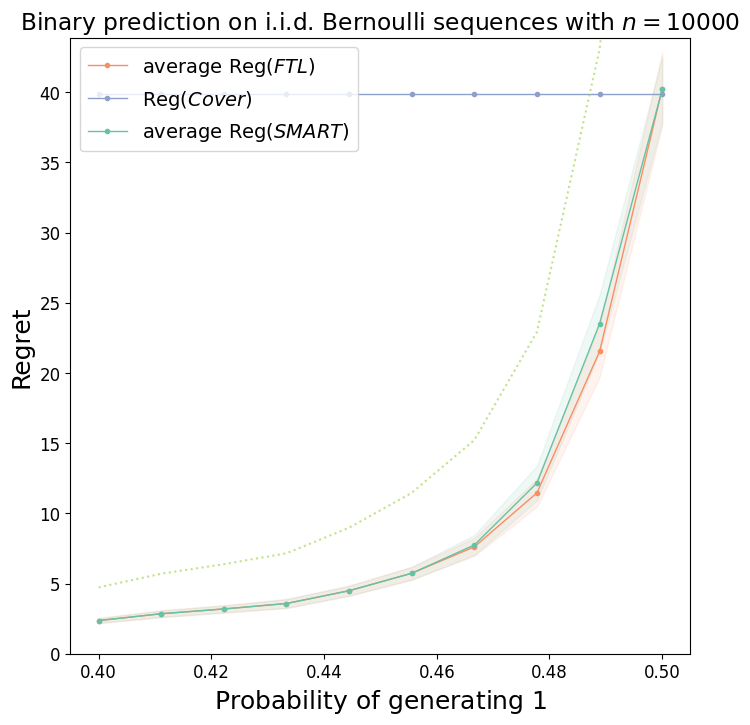
\includegraphics[height=\linewidth]{figures/detSMART_iid.png}
    %\caption{\it\scriptsize (a) $\bob$ with deterministic $\theta$, i.i.d. $y^n$}
  \end{minipage}%
  \hfill
  \begin{minipage}{.3\textwidth} % Adjust the width as needed
    \centering
    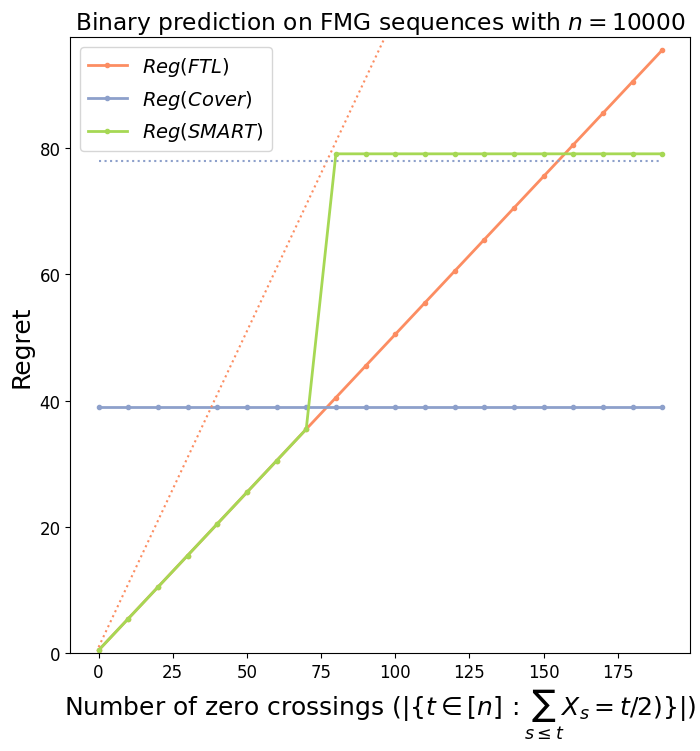
\includegraphics[height=\linewidth]{figures/detSMART_FMG.png}
    %\caption{\it\scriptsize (b) $\bob$ with deterministic $\theta$: FMG $y^n$}
  \end{minipage}%
  \hfill
  \begin{minipage}{.3\textwidth} % Adjust the width as needed
    \centering
    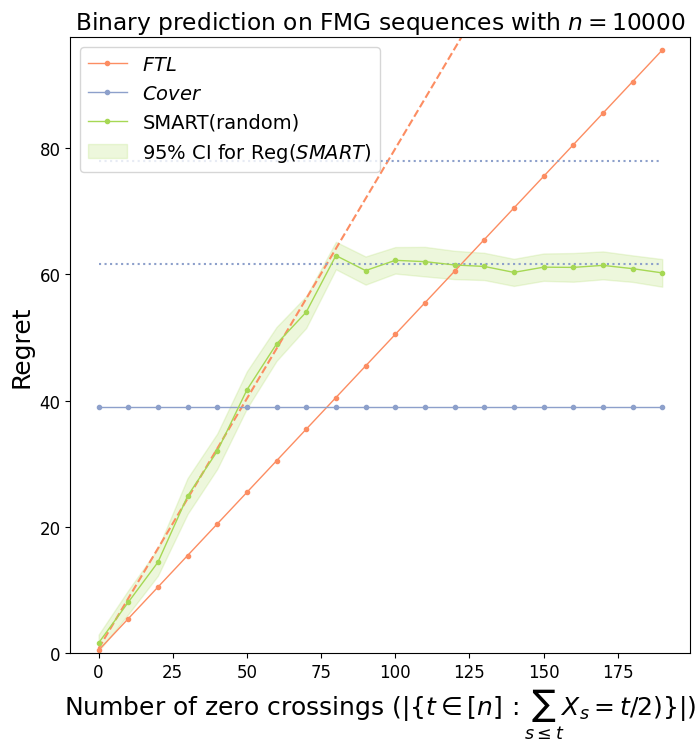
\includegraphics[height=\linewidth]{figures/randomSMART_FMG.png}
    %\caption{\it\scriptsize (c) $\bob$ with randomized $\theta$, FMG $y^n$}
  \end{minipage}
\captionsetup{format=plain}
  \caption{\it\footnotesize Comparing regret of $\ftl$, $\cover$ and $\bob$ on a collection of input sequences (for fixed $n$).\\ 
  $\bullet$ In Fig. $(a)$, we consider i.i.d. Bernoulli$(p)$ inputs for varying $p$. The regret of $\ftl$ is much lower than $\cover$ for $p<1/2$; the regret of $\bob$ tracks $\ftl$ closely (better than $2\Reg(\ftl)$, indicated by dotted line).\\
  $\bullet$ In Fig. $(b)$ and $(c)$, we consider `worst-case' binary sequences (as per~\citep{feder1992universal}) parameterized by the number of `lead-changes': the sequence with parameter $c$ comprises of $c$ pairs `$0,1$' or `$1,0$', followed by $n-2c$ `$1$'s. 
  %$\Reg(\ftl)$ on the sequence with $c$-crossings is $c/2$, while $\Reg(\cover)$ is constant ($\approx\sqrt{\frac{n}{2 \pi}}$). 
  In Fig. $(b)$, we consider $\bob$ with a deterministic switching threshold (\cref{thm:2ApproxRegret}) and compare $\Reg(\bob)$ with $2\Reg(\ftl)$ and $2\Reg(\cover)$ (dotted lines); in Fig. $(c)$, we use a randomized threshold (\cref{thm:SkiRentalRegret}), and show the average regret over the randomized threshold, as well as sample paths (plotted in green), and compare with $\frac{e}{e-1}$ times $\Reg(\ftl)$ and $\Reg(\cover)$ (dotted lines).}
  \label{fig:SMART}
  \vspace{-0.5cm}  
\end{figure}

We consider a general online learning setting where at the beginning of each round $t \in [n]$, a policy $\alg$ first plays an action $a_t \in \Ac$, following which, a loss function $\ell_t:\Ac\to [0,1]$ is revealed, resulting in a loss of $\ell_t(a_t)$. The \emph{regret} is defined according to:
\begin{align}
\label{eq:RegDefnGeneral}
    \Reg(\alg,\ell^n) = \textstyle\sum_{t=1}^n \ell_t(a_t) - \inf_{a \in \Ac} \textstyle\sum_{t=1}^n \ell_t(a).
\end{align} 
More generally, as in with bit prediction, we allow $\alg$ to play in round $t$ a measure $w_t\in\Delta_{\Ac}$ (i.e., play $\{w_t:\Ac\mapsto[0,1]|\sum_{a\in\Ac}w_t(a)=1\}$), resulting in an expected loss of $\sum_{a\in\Ac}w_t(a)\ell_t(a)$. For notational convenience, we henceforth use $(a_t,\ell_t(a_t))$ for the action/loss, and reserve use of expectations for randomness in the algorithm and/or sequence.

We want to understand when is it possible to attain instance optimality as in Eq.~\eqref{eq:instanceopt_binary} with respect to a given pair of algorithms. Ideally, we want the first to be optimal for stochastic instances, and the second to be minimax optimal; unfortunately however exact optimal policies are unknown except in simple settings. To this end, we make two amendments to our goal: First, for the stochastic optimal policy, we use $\ftl$; this is well defined in any online learning setting, and moreover, known to be optimal or near-optimal for a wide range of settings under minimal assumptions~\citep{kotlowski2018minimaxity}. Second, instead of the minimax policy, we use as reference \emph{any} policy $\wcalg$ which has a known worst case regret bound $g(n)$. With these modifications in place, we have the following objective.

%However, proving such a guarantee requires a tight characterization of the performance of both reference algorithms on every input sequence, which is not well understood for most algorithms. As a result, for general online learning, we consider the following weaker form of instance optimality
%with respect to the regret of $\ftl$ and a worst case regret bound $g(n)$.
\begin{definition} \label{def:instanceopt_wc}
Given $\ftl$ and any algorithm $\wcalg$ with $\sup_{\ell^n} \Reg(\wcalg, \ell^n) \le g(n)$, we say a policy $\alg$ is instance optimal with respect to the pair if there exists some universal $\gamma_n \geq 1$ such that for every sequence of losses $\ell^n$:
\begin{equation*}\label{eq:instanceopt_wc}
\small \Reg(\alg,\ell^n)\leq \gamma \min\{\Reg(\ftl,\ell^n),g(n)\}
\end{equation*}
%for all sequences of losses $\ell^n$. Equivalently, $\gamma$ is the competitive ratio achieved by $\alg$.
\end{definition}
While the above guarantee is not truly instance-optimal in that we are comparing against a worst-case regret bound $g(n)$ for $\wcalg$ rather than its performance on the instance $\ell^n$, the two are the same if $\wcalg$ is minimax optimal and hence attaining equal regret on all loss sequences; recall this is true of $\cover$  for binary prediction.

To realize the above goal, we propose the \emph{Switch via Monotone Adapted Regret Traces} ($\bob$) approach, which at a high level is a black-box way to convert design of instance-optimal policies into a simple \emph{optimal stopping} problem. 
Our approach depends on just two ingredients: first, owing to the additive structure of online learning problems, we have that the minimax guarantee $g(k)$ above holds over \emph{any} $k\in\mathbb{Z}$ and any (sub)sequence of $n$ loss functions; second, we show that $\ftl$ admits simple anytime regret estimator $\ftlsum_{\tau}$ (see Lemma~\ref{lem:FTLRegret}) which is \emph{monotone} and \emph{adapted} (i.e., a function only of historical data). Using these two observations, we can reduce the task of minimizing regret to a version of the `ski-rental' problem~\citep{karlin1994competitive,borodin2005online}, as follows:
we play $\ftl$ up to some stopping time $\tau$, and then switch to $\wcalg$ for the remaining $n-\tau$ periods, resetting all losses to zero. This algorithm  incurs a \emph{total} regret bounded by $\ftlsum_{\tau} + g(n-\tau)$, and using ideas from competitive analysis, we get that there is a simple way to choose the stopping time $\tau$ to achieve an $e/(e-1) \approx 1.58$-competitive ratio guarantee with respect to the minimum between the regret of $\ftl$ and the worst case guarantee $g(n)$.

%abbreviated statement
\begin{thm}{\emph{\bf (See Theorem~\ref{thm:SkiRentalRegret})}}
      Let $\wcalg$ have worst-case regret $\sup_{\ell^n} \Reg(\wcalg, \ell^n) \le g(n)$
      where $g(n)$ is some monotonic function of $n$. An instantiation of $\bob$ achieves  
    \begin{align} \label{eq:2ApproxReg}
\small        \Reg(\bob, \ell^n) \le \frac{e}{e-1} \min\{\Reg(\ftl,\ell^n),g(n)\} + 1.
    \end{align}
\end{thm}
A highlight of our approach is the surprising simplicity of the algorithm and analysis, despite the strength of the instance optimality guarantee. In particular, our approach is modular, allowing one to plug in any $\wcalg$ and corresponding worst case bound $g(n)$, thus letting us handle any online learning setting with known minimax bounds. This results in an entire family of instance optimal policies for settings such as predictions with experts and online convex optimization. Moreover, the approach is easy to extend to get more complex guarantees; as an example, if $\wcalg$ is designed to get low regret for benign (i.e., `small-loss') sequences $\ell^n$, then we show how to use $\bob$ as a subroutine and achieve an instance optimal guarantee with respect to the regret of $\ftl$ and a small loss regret bound. 
\begin{corollary}[Following Theorem~\ref{thm:Regret_small_loss}]
\label{cor:SqrtLStarInstantiation}
    Let $L^* \defeq \min_j \sum_{t=1}^n \ell_{tj}$. An instantiation of $\bob$ achieves
    \begin{align*}
    %\label{eq:BOBWSqrtLstarRegDoubling}
        % \Reg(\pstar, \ell^n) &\le 2 \min\left\{\Reg(\ftl, \ell^n), 8 \sqrt{2L^* \log m} + \kappa\log\left(1+\frac{L^*}{\log m}\right)\log m + 8\sqrt{2}\log m \right\} \nonumber\\
        % &\qquad\qquad\qquad\qquad\qquad+ 2 \log\left(1+ \frac{L^*}{\log m}\right)
        \Reg(\bob, \ell^n) 
        &\le 2 \min\left\{ \Reg(\ftl,\ell^n), 10 \sqrt{2L^* \log m} \right\} + O(\log L^* \log m).
    \end{align*}
\end{corollary}

Finally, studying instance optimality also lets us understand the fundamental limits of best-of-both worlds algorithms.
To this end, we provide a lower bound that shows our algorithm is nearly optimal in the competitive ratio. 
To the best of our knowledge, this is the first hardness result for best-of-both-worlds guarantees in online learning.
\begin{thm}{\emph{\bf (See Theorem~\ref{thm:LowerBdCR})}}
In the binary prediction setting, given \emph{any} online algorithm $\alg$, there exist sequences $y^n\in\{0,1\}^n$ such that:
\begin{align*}
    \Reg(\alg,y^n)
    &\geq 1.43\min\left\{\Reg(\ftl,y^n),\Reg(\cover,y^n)\right\}
\end{align*}
\end{thm}
Note again that in binary prediction, $\ftl$ achieves the optimal pseudoregret under i.i.d. inputs, while $\cover$ is the true minimax policy; thus, this is a fundamental lower bound on best-of-both-worlds guarantee in any online learning setting.

